\input{src/header}											% bindet Header ein (WICHTIG)
\usepackage{graphicx}
\usepackage{fancyvrb}

\newcommand{\dozent}{Prof. Dr. Agn`es Voisard, Nicolas Lehmann}					% <-- Names des Dozenten eintragen
\newcommand{\tutor}{Nicolas Lehmann}						% <-- Name eurer Tutoriun eintragen
\newcommand{\tutoriumNo}{10}				% <-- Nummer im KVV nachschauen
\newcommand{\projectNo}{2}									% <-- Nummer des Übungszettels
\newcommand{\veranstaltung}{Datenbanksysteme}	% <-- Name der Lehrveranstaltung eintragen
\newcommand{\semester}{SoSe 2017}						% <-- z.B. SoSe 17, WiSe 17/18
\newcommand{\studenten}{Boyan Hristov, Julian Habib}			% <-- Hier eure Namen eintragen
% /////////////////////// BEGIN DOKUMENT /////////////////////////


\begin{document}
% /////////////////////// BEGIN TITLEPAGE /////////////////////////
\begin{titlepage}
	\subject{\dozent}
	\title{\veranstaltung, \semester}
	\subtitle{\Large Übungsblatt \projectNo\\ \large\vspace{1ex} }
	\author{\studenten}
	\date{\normalsize \today}
\end{titlepage}

\maketitle								% Erstellt das Titelblatt
\vspace*{-9cm}							% rückt Logo an den oberen Seitenrand
\makebox[\dimexpr\textwidth+1cm][r]{	%rechtsbündig und geht rechts 1cm über Layout hinaus
	\includegraphics[width=0.4\textwidth]{src/fu_logo} % fügt FU-Logo ein
}
% /////////////////////// END TITLEPAGE /////////////////////////

\vspace{7cm}							% Abstand
\rule{\linewidth}{0.8pt}				% horizontale Linie										% erstellt die Titelseite


Link zum Git Repository: \url{https://github.com/BoyanH/Freie-Universitaet-Berlin/tree/master/Datenbanksysteme/Solutions/homework3}

% /////////////////////// Aufgabe 1 /////////////////////////
\section{Aufgabe}


\begin{itemize}

\item[a)]

Relationales Modell \\

% Relational Modell
\begin{Verbatim}[commandchars=+\[\]]

Person(+underline[ID::integer], Age::integer, Name::character varying(20), Password::character varying(40),
	Login::character varying(40))
Teacher(+underline[ID::integer])
Student(+underline[ID::integer])
Course(+underline[Number::integer], Name :: character varying(50))
Module(+underline[Number::integer], Name :: character varying(50))

PersonIsATeacher(+underline[PersonID, TeacherID])
PersonIsAStudent(+underline[PersonID, StudentID])
TeachesCourses(+underline[PersonID, CourseNumber], InSemester)
ContainsCourses(+underline[ModuleNumber, CourseNumber])
AttendsCourses(+underline[StudentID, CourseNumber])
\end{Verbatim}
% End of relational Modell

ER Diagramm in umgekehrter min-max Chen Notation \\

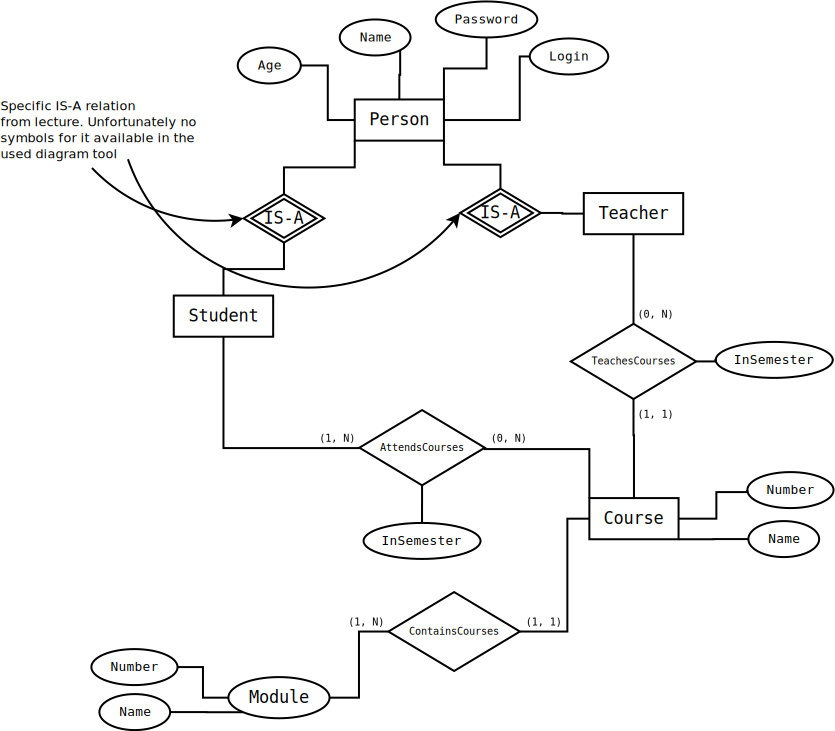
\includegraphics[width=\textwidth]{./src/exercise3_A.png}


\item[b)] 

Relationales Modell \\

% Relational Modell
\begin{Verbatim}[commandchars=+\[\]]

Person(+underline[ID::integer], Name::character varying(20))
Doctor(+underline[ID::integer], Specialty::character varying(30), Name::character varying(20))
Patient(+underline[ID::integer], HealthHistory::character varying(40) ARRAY, Name::character varying(20))
DoctorsAppointment(+underline[ID::integer], Date::date)
Address(+underline[PrivateAddressStreet::character varying(20)], City::character varying(20), 
	ServiceAddressStreet::character varying(20))

LivesIn(+underline[PersonID, AddressPrivateAdressStreet])
Attends(+underline[PersonID, DoctorsAppointmentID])
Services(+underline[PersonID, DoctorsAppointmentID])
\end{Verbatim}
% End of relational Modell

ER Diagramm in umgekehrter min-max Chen Notation\\

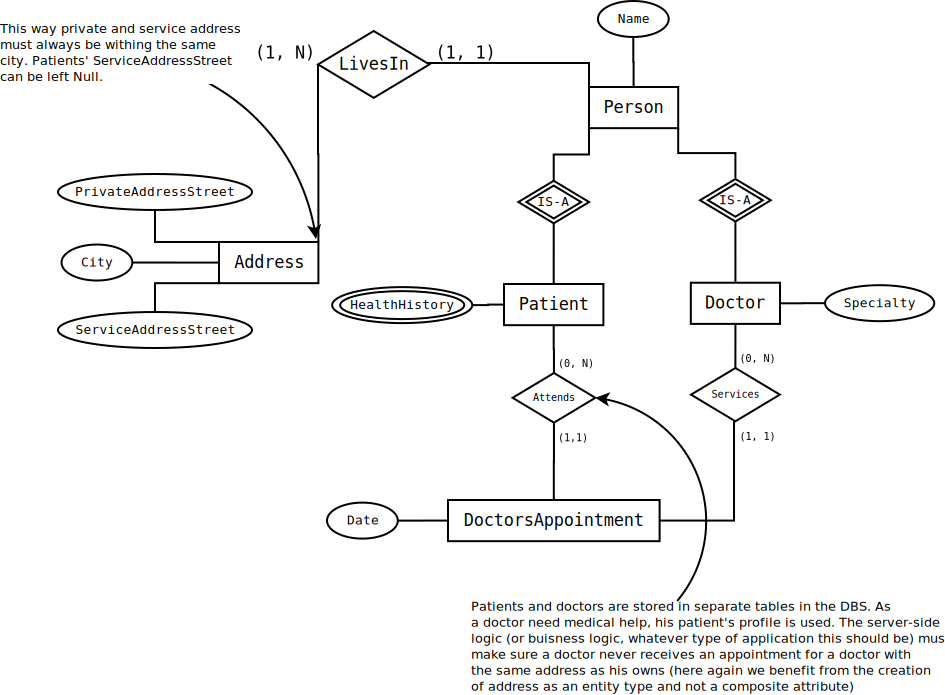
\includegraphics[width=\textwidth]{./src/exercise3_B.png}

\end{itemize}

\section{Aufgabe}

\begin{itemize}


\item[a)]
$\Pi_{\text{Vorname, Nachname}}$ ($\sigma_{\text{Alter} < 30 }$ (Passagier))

\item[b)]
$\Pi_{\text{Datum}}$ ($\sigma_{\text{Temperatur > Regenmenge } \lor \text{ Temperatur > Sonnenscheindauer} }$ (Wetter))

\item[c)]
$\Pi_{\text{Kreditkartennummer}}$ ($\sigma_{\text{Name = 'Emirates' $\land$ Datum $\geq$ '02.03.2016' $\land$ Datum $\leq$ '07.06.2016'}}$  (Passagier $\bowtie_{\text{ID = Passagier-ID}}$ Flug $\bowtie_{\text{Fluggesellschaft-ID = ID}}$ Fluggesellschaft))

\item[d)]
$\Pi_{\text{Name}}$ ($\sigma_{\text{Temperatur < 0}}$ (Wetter $\bowtie_{\text{Wetter::Datum = Flug::Datum}}$ Flug $\bowtie_{\text{Fluggesellschaft-ID = ID}}$ Fluggesellschaft))

\item[e)]
$\Pi_{\text{Vorname, Nachname}}$ ($\sigma_{\neg\text{(Temperatur < 20 $\land$ Regenmenge > 10 $\land$ Sonnenscheindauer < 6)}}$ (Wetter $\bowtie_{\text{Wetter::Datum = Flug::Datum}}$ Flug $\bowtie_{\text{Passagier-ID = ID}}$ Passagier))

\end{itemize}

\section{Aufgabe}

Um die Aufgabe richtig zu lösen, muss man Attribute (Spalten) umbenennen können. Sonst kann man nicht äußern, dass z.B. Nachname und Datum gleich sein müssen, ID aber nicht. 
Nach der Annahme, dass wir die Operation zum Umbenennen benutzen können, kann man die Folgende aufgaben so lösen (Diese Operation ist offiziel in der relationalen Algebra enthalten). \\

Wir haben die einzelne Teile in separate Queries geteilt, damit man besser verstehen kann was genau passiert.

\begin{itemize}

\item[a)]

q1 = $\sigma_{text{Alter > 30}}$ (Passagier $\bowtie_{\text{ID = Passagier-ID}}$ Flug) \\
q2 = $\Pi_{\text{Vorname, Nachname, Datum, Fluggesellschaft-ID}}$ (q1) \\
q3 = q2 $\bowtie (\delta$ 'Vorname' $\rightarrow$ 'Vorname-duplicate' q2) \\
q4 = q3 - $\sigma_{\text{Vorname = Vorname-duplicate}} (q3)$ \\
q5 = $\Pi_{\text{Vorname, Nachname}}$ (q4) \\

q1 nimmt alle Passagiere, die über 30 Jahre alt sind und die dazugehörige Fluge.
q2 nimmt nur die Attributen Vorname, Nachname, Datum und Fluggesellschaft-ID davon. Dies wird gemacht, damit dann bei q3 alle mögliche Kombinationen von Passagieren, die im selben Flug geflogen sind und die selbe Nachname haben (wir haben angenommen, das ein Flug durch Datum und Fluggesellschaft-ID eindeutig charakterisiert wird) erzeugt werden. Dann sorgt q4 dass Entitäten mit gleiche Vorname und Vorname-duplicate gelöscht werden. Fall mindestends 2 Personen mit dem selben Nachname gibt, dann gibt es mindestens 4 Entitäten, die originelle und diese mit vertauschte Vorname und Vorname-duplicate. Nur diese mit vertauschte (unterschiedliche) Vorname und Vorname-duplicate werden im q4 selektiert. Danach wird in q5 die Vorname und Nachname dieser Entitäten selektiert.

\item[b)]

q1 = Passagier $\bowtie_{\text{ID = Passagier-ID}}$ Flug \\
q2 = $\Pi_{\text{Alter, Datum, Fluggesellschaft-ID}}$ (q1) \\
q3 = q2 $\bowtie (\delta$ 'Alter' $\rightarrow$ 'Alter-duplicate' q2) \\
q4 = q2 - $\sigma_{\text{Alter = Alter-duplicate}}$ (q2) \\
q5 = $\Pi_{\text{Datum, Fluggesellschaft-ID}}$ (q4) \\
q6 = q1 - q5 \\
q7 = $\Pi_{\text{Datum, Fluggesellschaftsname}}$ (q6 $\bowtie_{\text{FluggesellschaftID = ID}}$ Fluggesellschaft) \\

Nach der selben Logik haben wir in q4 Alle Flüge, auf dem mindestens zwei Personen das selbe Alter haben. In q5 nehmen wir nur Datum und Fulggesellschaft-ID (Das Superkey einer Flug, nach Annahme) damit wir in q6 alle Flüge bekommen können, die nur Passagiere mit verschiedenem Alter haben. Dann wird in q7 die Fluggesellschaft Tabelle dazugenommen, damit Datum und Fluggesellschaftsname zurückgegeben werden können. \\ \\

Quelle - eine analoge Frage im StackOverflow: \url{https://stackoverflow.com/questions/43567351/relational-algebra-natural-join-of-table-q2-with-rename-of-table-q2-for-passenge}

\section{Aufgabe}

\begin{lstlisting}

<!DOCTYPE html>
<html>
<head>
	<meta charset="utf-8"></meta>
	<title>Apple Aktie</title>
	<style type="text/css">

		#linechart, #barchart {

			width: 600px;
			height: 400px;
		}

	</style>
	<script type="text/javascript" language="javascript" src="./bower_components/jquery/dist/jquery.min.js"></script>
	<script type="text/javascript" language="javascript" src="./bower_components/Flot/jquery.flot.js"></script>
</head>
<body>
	<div id="linechart"></div>
	<div id="barchart"></div>
	<script type="text/javascript">

		function parseDataToObject(data) {

			var rows = data.split('\r\n').map(function (item) {
				return item.replace(';', '').split(',');
			});
			var attributes = rows[0];
			var parsedObject = {};

			rows = rows.slice(1);
			attributes.forEach(function (attr, idx) {

				parsedObject[attr] = rows.map(function (row) {
					
					if(attr === 'Datum') {
				
						var crntDate = new Date(),
							crntDecade = crntDate.getFullYear().toString().slice(0,2);
							valueArr = row[idx].split('.'),
							day = valueArr[0]*1,
							month = valueArr[1]*1 - 1,
							year = (crntDecade + valueArr[2])*1,
							date = new Date(year, month, day);

						return date.getDate()*1;
					}
					return row[idx]*1;
				});
			});

			return parsedObject;
		}

		function mergeArrayEntities(arrA, arrB) {

			var copyA = arrA.slice(0),
				copyB = arrB.slice(0);

			if(copyA.length !== copyB.length) {

				throw new Error('Only arrays with equal length can be merged!');
			}

			return copyA.map(function (item, idx) {

				return [item, copyB[idx]];
			});
		}

		$.get('./data/apple.csv', function(data) {

			var parsedData = parseDataToObject(data);
			
			$.plot($('#linechart'), 
				[

					{color: '#f00', data: mergeArrayEntities(parsedData.Datum, parsedData.Tief)},
					{color: '#0f0', data: mergeArrayEntities(parsedData.Datum, parsedData.Hoch)},
					{color: '#ff0', data: mergeArrayEntities(parsedData.Datum, parsedData.Tagesendwert)}

			]);

			$.plot($('#barchart'), 
				[

					{color: '#f00', data: mergeArrayEntities(parsedData.Datum, parsedData.Handelsvolumen)}

				], 
				{
		            series: {
		                bars: {
		                    show: true
		                }
		            },
		            bars: {
		                align: "center",
		                barWidth: 0.5
		            }
			});

		});

	</script>
</body>
</html>

\end{lstlisting}


\end{itemize}




% /////////////////////// END DOKUMENT /////////////////////////
\end{document}
